\documentclass[12pt,a4paper,openany]{article}
\usepackage[utf8]{inputenc}
\usepackage[T1]{fontenc}
\usepackage[spanish]{babel}
\usepackage{amsmath}
\usepackage{amsfonts}
\usepackage{amssymb}
\usepackage{graphicx}
\usepackage{float}
\usepackage[breaklinks=true]{hyperref}
\author{Luis Alberto López Durán}
\title{Campo magnético rotativo}
\spanishdecimal{.}

\begin{document}
	\maketitle
	
	\section{Introducción}
	El principio de funcionamiento fundamental de los motores de corriente alterna es que si \textit{un grupo de tres señales senoidales de igual magnitud, pero cada una desplazada 120° entre sí fluyen en un devanado trifásico, producirán un campo magnético giratorio de magnitud constante}. \cite{chapman}
	
	Ya que el concepto de campo magnético rotativo (CMR) es tan importante para el entendimiento de las máquinas de \textit{ca}, resulta apropiado realizar un análisis del mismo, por esta razón se realiza este trabajo, con la finalidad de entender el concepto, así como mostrar una simulación desarrollada en el software LabVIEW a fin de ilustrar de mejor manera este tema.
	
	\section{Antecedentes}
	La primera aparición de los principios del concepto de campo magnético rotativo tuvo lugar en 1885 por parte de Galileo Ferraris, un profesor de la Universidad de Turín, quien descubrió que dos corrientes alternas actuando simultáneamente sobre dos devanados colocados en el estátor de una máquina eléctrica producen en su interior un campo magnético giratorio capaz de arrastrar un rotor con un cilindro de cobre, siempre que se cumpla la condición de que las dos corrientes estén desfasadas en el tiempo y los dos devanados desplazados en el espacio. Ferraris, sin embargo, no concedió importancia a su descubrimiento, e incluso llegó a afirmar que no servía para construir nuevos modelos de motores eléctricos suficientemente eficaces.
	
	No sería hasta el año de 1887 en que Nikola Tesla y Mikhail Osipovich Dolivo-Dobrovolsky en 1889 que sentaron completamente las bases para este concepto, cuando presentaron un motor de inducción bajo estos principios. \cite{internet}
	
	
	\section{Campo magnético rotativo (CMR)}
	Para comenzar a entender el concepto de CMR recordemos que este se da a partir de tres señales senoidales de corriente defasadas 120° entre sí, haciendo entonces que tales señales correspondan a:
	
	\begin{equation*}
		i_{aa'}(t)=I_{M}\sin \omega t \quad A
	\end{equation*}
	\begin{equation*}
		i_{bb'}(t)=I_{M}\sin (\omega t - 120^{\circ}) \quad A
	\end{equation*}
	\begin{equation*}
		i_{cc'}(t)=I_{M}\sin (\omega t - 240^{\circ}) \quad A
	\end{equation*}
	\\
	Donde los subíndices \textit{aa'}, \textit{bb'} y \textit{cc'} corresponden a los extremos de los devanados, tomando en cuenta que hay seis bobinas que se conectan de dos en dos, en el devanado \textit{A}, un extremo corresponde a \textit{a}, por el que entra la corriente y el otro a \textit{a'}, por el que sale, lo mismo pasa para los otros devanados. El factor $I_M$ corresponde a la amplitud máxima de la señal de corriente.
	
	El flujo de estas corrientes produce, entonces, intensidades de campo magnético, recordando que $H_M$ es la magnitud máxima de la intensidad de campo magnético.
	
	\begin{equation*}
		\mathbf{H}_{aa'}(t)=H_{M}\sin \omega t \angle{0^{\circ}} \quad A \cdot vuelta/m
	\end{equation*}
	\begin{equation*}
		\mathbf{H}_{bb'}(t)=H_{M}\sin (\omega t - 120^{\circ}) \angle{120^{\circ}} \quad A \cdot vuelta/m
	\end{equation*}
	\begin{equation*}
		\mathbf{H}_{cc'}(t)=H_{M}\sin (\omega t - 240^{\circ})  \angle{240^{\circ}} \quad A \cdot vuelta/m
	\end{equation*}
	\\
	Y las densidades de flujo de las intensidades anteriores se obtienen de la ecuación que nos dice que $\mathbf{B}=\mu \mathbf{H}$, y de esta manera:
	
	\begin{equation*}
		\mathbf{B}_{aa'}(t)=B_{M}\sin \omega t \angle{0^{\circ}} \quad T
	\end{equation*}
	\begin{equation*}
		\mathbf{B}_{bb'}(t)=B_{M}\sin (\omega t - 120°) \angle{120^{\circ}} \quad T
	\end{equation*}
	\begin{equation*}
		\mathbf{B}_{cc'}(t)=B_{M}\sin (\omega t - 240°) \angle{240^{\circ}} \quad T
	\end{equation*}
	\\
	Donde $B_M$ es la magnitud máxima de la densidad de flujo magnético.
	
	Con estas últimas expresiones obtenidas, de la densidad de campo magnético, podemos encontrar el vector resultante en ciertos intervalos de tiempo, haremos, pues, el ejemplo para cuando $\omega t= 0^{\circ}$ y $\omega t= 90^{\circ}$. Comenzaremos con el primero.

	\begin{equation*}
		\mathbf{B}_{aa'}(t)=B_{M}\sin 0^{\circ} \angle{0^{\circ}} \quad T
	\end{equation*}
	\begin{equation*}
		\mathbf{B}_{bb'}(t)=B_{M}\sin (- 120^{\circ}) \angle{120^{\circ}} \quad T
	\end{equation*}
	\begin{equation*}
		\mathbf{B}_{cc'}(t)=B_{M}\sin (- 240^{\circ}) \angle{240^{\circ}} \quad T
	\end{equation*}	
	\\
	Y al sumarlas para encontrar el vector resultante obtenemos lo siguiente:
	
	\begin{equation*}
		\mathbf{B}_{net}=\mathbf{B_{aa'}} + \mathbf{B_{bb'}} + \mathbf{B_{cc'}}
	\end{equation*}	
	
	\begin{equation*}
		\mathbf{B}_{net}=0-\left(\frac{\sqrt{3}}{2} B_{M}\right)\left(\cos120^{\circ}\mathbf{\hat{x}}+\sin120^{\circ}\mathbf{\hat{y}}\right)+\left(\frac{\sqrt{3}}{2} B_{M}\right)\left(\cos240^{\circ}\mathbf{\hat{x}}+\sin240^{\circ}\mathbf{\hat{y}}\right)
	\end{equation*}
	
	\begin{equation*}
		\mathbf{B}_{net}=\left(\frac{\sqrt{3}}{2} B_{M}\right)\left[-\left(\cos120^{\circ}\mathbf{\hat{x}}+\sin120^{\circ}\mathbf{\hat{y}}\right)+\left(\cos240^{\circ}\mathbf{\hat{x}}+\sin240^{\circ}\mathbf{\hat{y}}\right)\right]
	\end{equation*}
	
	\begin{equation*}
		\mathbf{B}_{net}=\left(\frac{\sqrt{3}}{2} B_{M}\right)\left( \frac{1}{2}\mathbf{\hat{x}}-\frac{\sqrt{3}}{2}\mathbf{\hat{y}}-\frac{1}{2}\mathbf{\hat{x}}-\frac{\sqrt{3}}{2}\mathbf{\hat{y}} \right)
	\end{equation*}
	
	\begin{equation*}
		\mathbf{B}_{net}=\left(\frac{\sqrt{3}}{2} B_{M}\right)\left( -\frac{\sqrt{3}}{2}\mathbf{\hat{y}}-\frac{\sqrt{3}}{2}\mathbf{\hat{y}} \right)
	\end{equation*}
	
	\begin{equation*}
		\mathbf{B}_{net}=\left(\frac{\sqrt{3}}{2} B_{M}\right)\left( -\sqrt{3}\mathbf{\hat{y}} \right)
	\end{equation*}
	
	\begin{equation*}
		\mathbf{B}_{net}=-\frac{3}{2}B_M\mathbf{\hat{y}}
	\end{equation*}
	
	\begin{equation*}
		\mathbf{B}_{net}=-1.5B_M\mathbf{\hat{y}}
	\end{equation*}
	
	\begin{equation*}
		\mathbf{B}_{net}=1.5B_M\angle{-90^{\circ}}
	\end{equation*}
	
	Ahora se encontrará el vector resultante de la densidad de campo magnético con $\omega t=90^{\circ}$.
	
	\begin{equation*}
	\mathbf{B}_{aa'}(t)=B_{M}\sin 90^{\circ} \angle{0^{\circ}} \quad T
	\end{equation*}
	\begin{equation*}
	\mathbf{B}_{bb'}(t)=B_{M}\sin (90^{\circ} - 120^{\circ}) \angle{120^{\circ}} \quad T
	\end{equation*}
	\begin{equation*}
	\mathbf{B}_{cc'}(t)=B_{M}\sin (90^{\circ} - 240^{\circ}) \angle{240^{\circ}} \quad T
	\end{equation*}	
	\\
	Y al sumarlas para encontrar el vector resultante obtenemos lo siguiente:
	
	\begin{equation*}
		\mathbf{B}_{net}=B_M\mathbf{\hat{x}}-\left(\frac{1}{2}B_M\right)\left(\cos120^{\circ}\mathbf{\hat{x}}+\sin120^{\circ}\mathbf{\hat{y}}\right)-\left(\frac{1}{2}B_M\right)\left(\cos240^{\circ}\mathbf{\hat{x}}+\sin240^{\circ}\mathbf{\hat{y}}\right)
	\end{equation*}
	
	\begin{equation*}
		\mathbf{B}_{net}=B_M\mathbf{\hat{x}}-\left(\frac{1}{2}B_M\right)\left(-\frac{1}{2}\mathbf{\hat{x}}+\frac{\sqrt{3}}{2}\mathbf{\hat{y}}\right)-\left(\frac{1}{2}B_M\right)\left(-\frac{1}{2}\mathbf{\hat{x}}-\frac{\sqrt{3}}{2}\mathbf{\hat{y}}\right)
	\end{equation*}
	
	\begin{equation*}
		\mathbf{B}_{net}=\left[\mathbf{\hat{x}}-\left(-\frac{1}{4}\mathbf{\hat{x}}+\frac{\sqrt{3}}{4}\mathbf{\hat{y}}\right)-\left(-\frac{1}{4}\mathbf{\hat{x}}-\frac{\sqrt{3}}{4}\mathbf{\hat{y}}\right)\right]B_M
	\end{equation*}
	
	\begin{equation*}
		\mathbf{B}_{net}=\left(\mathbf{\hat{x}}+\frac{1}{4}\mathbf{\hat{x}}-\frac{\sqrt{3}}{4}\mathbf{\hat{y}}+\frac{1}{4}\mathbf{\hat{x}}+\frac{\sqrt{3}}{4}\mathbf{\hat{y}}\right)B_M
	\end{equation*}
	
	\begin{equation*}
		\mathbf{B}_{net}=\frac{3}{2}B_M\mathbf{\hat{x}}
	\end{equation*}
	
	\begin{equation*}
		\mathbf{B}_{net}=1.5B_M\mathbf{\hat{x}}
	\end{equation*}
	
	\begin{equation*}
		\mathbf{B}_{net}=1.5B_M\angle{0^\circ}
	\end{equation*}
	\\
	Recordando los resultados a los que llegamos, para $\omega t=0^{\circ}$, $\mathbf{B}_{net}=1.5B_M\angle{-90^{\circ}}$ y para $\omega t=0^{\circ}$, $\mathbf{B}_{net}=1.5B_M\angle{0^\circ}$, lo que nos quiere decir que el sentido de giro del campo magnético resultante es contrario a las manecillas del reloj, como muestra la siguiente imagen, correspondiente a los análisis anteriores.
	
	\begin{figure}[H]
		\centering
		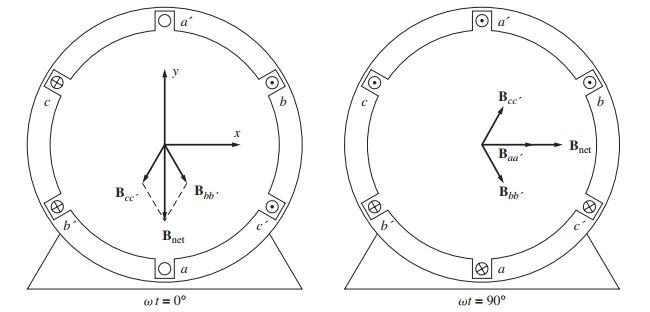
\includegraphics[width=1\linewidth]{Images/Campo_magnético_resultante_0_90}
		\caption{Campo magnético resultante para $\omega t=0^{\circ}$ y $\omega t=90^{\circ}$. \textit{Fuente: Máquinas Eléctricas, Quinta Edición - Stephen Chapman.}}
		\label{fig:campomagneticoresultante090}
	\end{figure}
	
	\section{Simulación en LabVIEW}
	Para demostrar de manera más gráfica e ilustrativa el concepto de CMR se simuló el comportamiento del campo magnético implementando las ecuaciones de la sección anterior. A continuación se presentan algunos de los resultados obtenidos.
	
	El diagrama de bloques resultó como se muestra a continuación, donde, mediante un nodo de fórmula se implementaron las expresiones para calcular el campo magnético resultante a partir de cada una de las tres densidades de campo magnético producidas por la señal de corriente alterna.
	
	\begin{figure}[H]
		\centering
		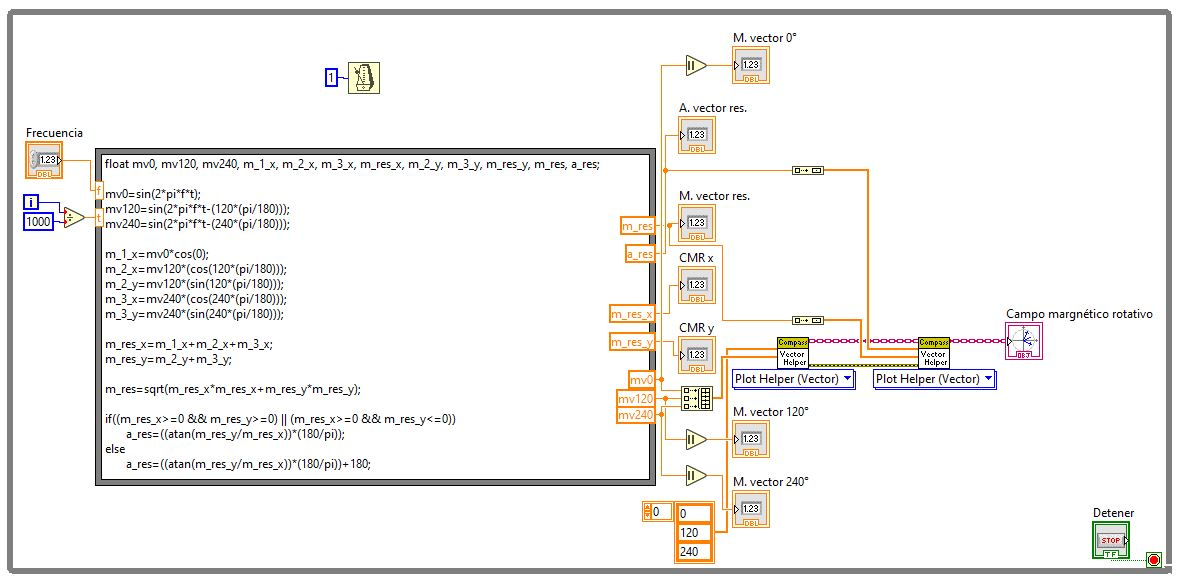
\includegraphics[width=0.75\linewidth]{Images/BlockDiagram}
		\caption{Diagrama de bloques para la simulación.}
		\label{fig:blockdiagram}
	\end{figure}
	
	Y como se puede observar en la vista del panel frontal de la simulación, el vector del CMR resultante se comporta de tal manera que nos esperaríamos con las operaciones teóricas, puesto que este vector se mueve en contra de las manecillas del reloj, como indica la Figura \href{fig:campomagneticoresultante090} 1.
	
	\begin{figure}[H]
		\centering
		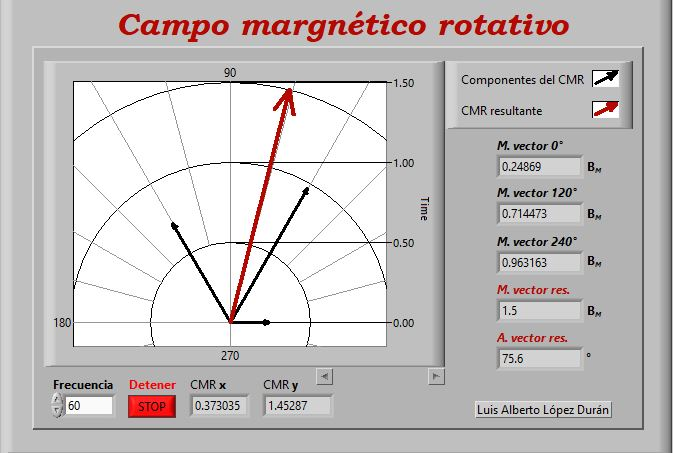
\includegraphics[width=0.6\linewidth]{Images/FrontPanel}
		\caption{Simulación del campo magnético rotativo.}
		\label{fig:frontpanel}
	\end{figure}
	
	\section{Conclusión}
	El concepto de campo magnético rotativo es uno de los que más han llamado mi atención de entre los temas que se han visto hasta el momento en la unidad respecto a máquinas de ca, del curso de Máquinas eléctricas, tal concepto me parece interesante y de suma importancia para entender el funcionamiento de las máquinas de ca, debido a que, es justamente este el principio fundamental de operación de dichas máquinas.
	
	A partir de los resultados alcanzados de manera teórica como simulada se concluye en un éxito de esta práctica, ya que coinciden entre ellos.
	
	Es interesante ver como en todo momento, independientemente del valor de la velocidad angular multiplicada por el tiempo ($\omega t$), la magnitud del vector resultante es siempre 1.5 veces la magnitud máxima que pueden alcanzar cada uno de los vectores de densidad de campo magnético de cada devanado, y es que es este, el principio que se requiere lograr para que una máquina de ca funcione, \textit{que se genere un campo magnético giratorio de magnitud constante}.
	
	\begin{thebibliography}{100}
		\bibitem{chapman}Chapman, S. \emph{"Máquinas eléctricas"}, Quinta edición, McGraw-Hill. 2021, México D.F.
		\bibitem{internet}Anónimo \emph{"Máquinas eléctricas: un poco de historia (1831-1900)"}, disponible en: \url{https://sites.google.com/site/espaciotesla/maquinas-electricas}
	\end{thebibliography}
	
\end{document}